% указываем класс документа
\documentclass[12pt,a4paper,openany]{extarticle}

% подключаем собственный стилевой файл 
\usepackage{mystyle}

% указываем язык (для автоматической вставки слов, типа "Глава", "Содержание", "Литература", "рис." и пр.
\selectlanguage{russian}

\begin{document}
\part*{Лабораторная работа №2\\
Получение конструктивных постоянных двигателя}
\section{Методические рекомендации}
До начала работы студент должен выполнить предыдущие работы этого цикла. Так~же необходимо ознакомиться с~представлением объектов управления в~пространстве состояний. Необходимо знание формул перехода между моделями ВСВ и ВВ.
\section{Теоретические сведения}
В предыдущей лабораторной работе нами рассмотрена упрощенная модель двигателя NXT. Но для~полной картины, необходимо получить зависимость угловой скорости двигателя от~подаваемого напряжения.
Для этого необходимо рассмотреть двигатель NXT с~учетом электрических процессов. Соответственно появится еще одна динамика, связанная с~индуктивностью обмотки двигателя. 

\begin{figure}[H]
	\noindent\centering{
		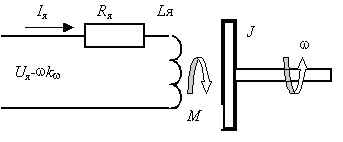
\includegraphics[scale=0.8]{engine_struct.jpg}
	}
	\caption{Структурная схема двигателя.}
	\label{fig:engine_struct}
\end{figure}

Запишем уравнение для~описания электрических процессов в~цепи с~учетом влияния противо"~ЭДС, создаваемым вращением якоря, учитывая $E_\textit{ЭДС}=\omega k_e$:
\begin{equation}
U_\textit{я}-E_\textit{ЭДС}=R_\textit{я}I+L_\textit{я}\frac{dI}{dt}\Rightarrow U_\textit{я}-\omega k_e=R_\textit{я}I+L_\textit{я}\frac{dI}{dt}
\end{equation}
Где $k_e$~--- конструктивная постоянная двигателя, связывающая угловую скорость и противо"~ЭДС. Теперь наша отрицательная обратная связь попадает не в~канал управления по~моменту, а прибавляется к~управляющему напряжению.

\begin{figure}[H]
	\noindent\centering{
		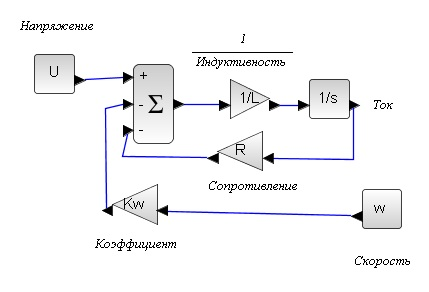
\includegraphics[scale=0.8]{engine_el_struct.jpg}
	}
	\caption{Структурная схема электрической цепи двигателя.}
	\label{fig:engine_el_struct}
\end{figure}

Надо отметить, что момент и ток в~цепи двигателя, так~же имеют линейную зависимость $M=k_mI$, где $k_m$~--- конструктивная постоянная двигателя, связывающая ток и момент (подробнее об~этом можно узнать в~курсе «Электрические машины»).Теперь запишем систему дифференциальных уравнений с~учетом формул, полученных в~прошлой лабораторной работе:
\begin{equation}
\left\{
\begin{aligned}
&\dot{\omega}=\frac{k_m}{J}I, \\
&\dot{I}=\frac{1}{L}U-\frac{k_e}{L}\omega-\frac{R_\textit{я}}{L}I.
\end{aligned}
\right.
\end{equation}
Записав эти уравнения, можно обозначить вектор состояния двигателя как $x=\begin{bmatrix}\omega\\I\end{bmatrix}$, соответственно можно записать эту систему уравнений в~матричном виде $\dot{x}=Ax+Bu$:
\begin{equation}
\begin{bmatrix}
\dot{\omega} \\ \dot{I}
\end{bmatrix}
=
\begin{bmatrix}
0 & \cfrac{k_m}{J} \\
-\cfrac{k_e}{L} & -\cfrac{R_\textit{я}}{L}
\end{bmatrix}
\begin{bmatrix}
\omega \\ I
\end{bmatrix}
+
\begin{bmatrix}
0 \\ \cfrac{1}{L}
\end{bmatrix}
U.
\end{equation}
Обратите внимание, если выполнить все арифметические действия с~матрицами, то мы получим исходную систему уравнений. Далее, из~записанного вида, мы можем получить передаточную функцию. Для~этого воспользуемся структурной схемой на~рисунке~\ref{fig:cond}.

\begin{figure}[H]
	\noindent\centering{
		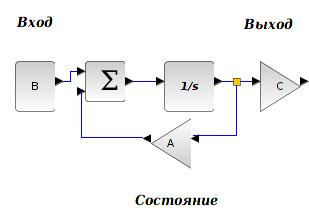
\includegraphics[scale=0.6]{cond.jpg}
	}
	\caption{Структурная схема электрической цепи двигателя.}
	\label{fig:cond}
\end{figure}

Запишем передаточную функцию системы, выразив ее уравнениями:
\begin{equation}
\left\{
\begin{aligned}
&\dot{X}=BU+AX,\\
&Y=C^TX.
\end{aligned}
\right.
\end{equation}
Применим преобразование Лапласа:
\begin{equation}
\left\{
\begin{aligned}
&sX=BU(s)+AX\Rightarrow X=(sI-A)^{-1}BU(s),\\
&Y(s)=C^T(sI-A)^{-1}BU(s)\Rightarrow W(s)=\frac{Y(s)}{U(s)}=C^T(sI-A)^{-1}B,
\end{aligned}
\right.
\end{equation}
где $I$~--- это единичная матрица. В~нашем случае матрица выхода равна $C^T=[1\;0]$, так~как на~выходе мы получаем угловую скорость.\\
Произведем соответствующие вычисления для~нашего случая:
\begin{eqnarray}
sI-A&=&
\begin{bmatrix}
s & - \cfrac{k_m}{J}\\
\cfrac{k_e}{L} & s+\cfrac{R_\textit{я}}{L}
\end{bmatrix}
,\quad(sI-A)^{-1}=\frac{1}{s^2+\cfrac{R_\textit{я}}{L}s+\cfrac{k_mk_e}{LJ}}
\begin{bmatrix}
s+\cfrac{R_\textit{я}}{L} & \cfrac{k_m}{J}\\
-\cfrac{k_e}{L} & s
\end{bmatrix}
,\\
W(s)&=&C(sI-A)^{-1}B=\frac{1}{s^2+\cfrac{R_\textit{я}}{L}s+\cfrac{k_mk_e}{LJ}}
\begin{bmatrix}
1 & 0
\end{bmatrix}
\begin{bmatrix}
s+\cfrac{R_\textit{я}}{L} & \cfrac{k_m}{J}\\
-\cfrac{k_e}{L} & s
\end{bmatrix}
\begin{bmatrix}
0\\
\cfrac{1}{L}
\end{bmatrix}
,\\
W(s)&=&\frac{\cfrac{k_m}{LJ}}{s^2+\cfrac{R_\textit{я}}{L}s+\cfrac{k_mk_e}{LJ}},\\
W(s)&=&\frac{1/k_e}{\cfrac{L}{R_\textit{я}}\cfrac{R_\textit{я}J}{k_mk_e}s^2+\cfrac{R_\textit{я}J}{k_mk_e}s+1}.
\end{eqnarray}
Где, $\cfrac{L}{R_\textit{я}}=T_e$~--- электромагнитная постоянная времени, $\cfrac{R_\textit{я}J}{k_mk_e}=T_m$~--- электромеханическая постоянная времени. Отметим, что $k_m=\cfrac{M_\textit{пуск}}{I}$, $k_e=\cfrac{E_\textit{ЭДС}}{\omega_0}$, подставим их в~электромеханическую постоянную времени $T_m=\cfrac{R_\textit{я}J}{\cfrac{M_\textit{пуск}}{I}\cfrac{E_\textit{ЭДС}}{\omega_0}}=\cfrac{J\omega_0}{M_\textit{пуск}}$. То~же, что мы получили в~прошлой лабораторной работе, рассматривая упрощенную модель. В~итоге получим:
\begin{equation}
W(s)=\frac{1/k_e}{T_eT_ms^2+T_ms+1}.
\end{equation}
\newpage
\section{Цель работы}
Определить конструктивные постоянные двигателя. Для~этого нужно измерить сопротивление обмотки якоря $R_\textit{я}$ и момент инерции двигателя~$J$.
Снять показания тока и напряжения. Далее, используя значение $T_m$, полученное в~первой лабораторной работе, рассчитать конструктивные постоянные двигателя. Значения угловой скорости ротора двигателя нужно брать в 48 раз больше, ввиду наличия редуктора.
\begin{figure}[H]
	\noindent\centering{
		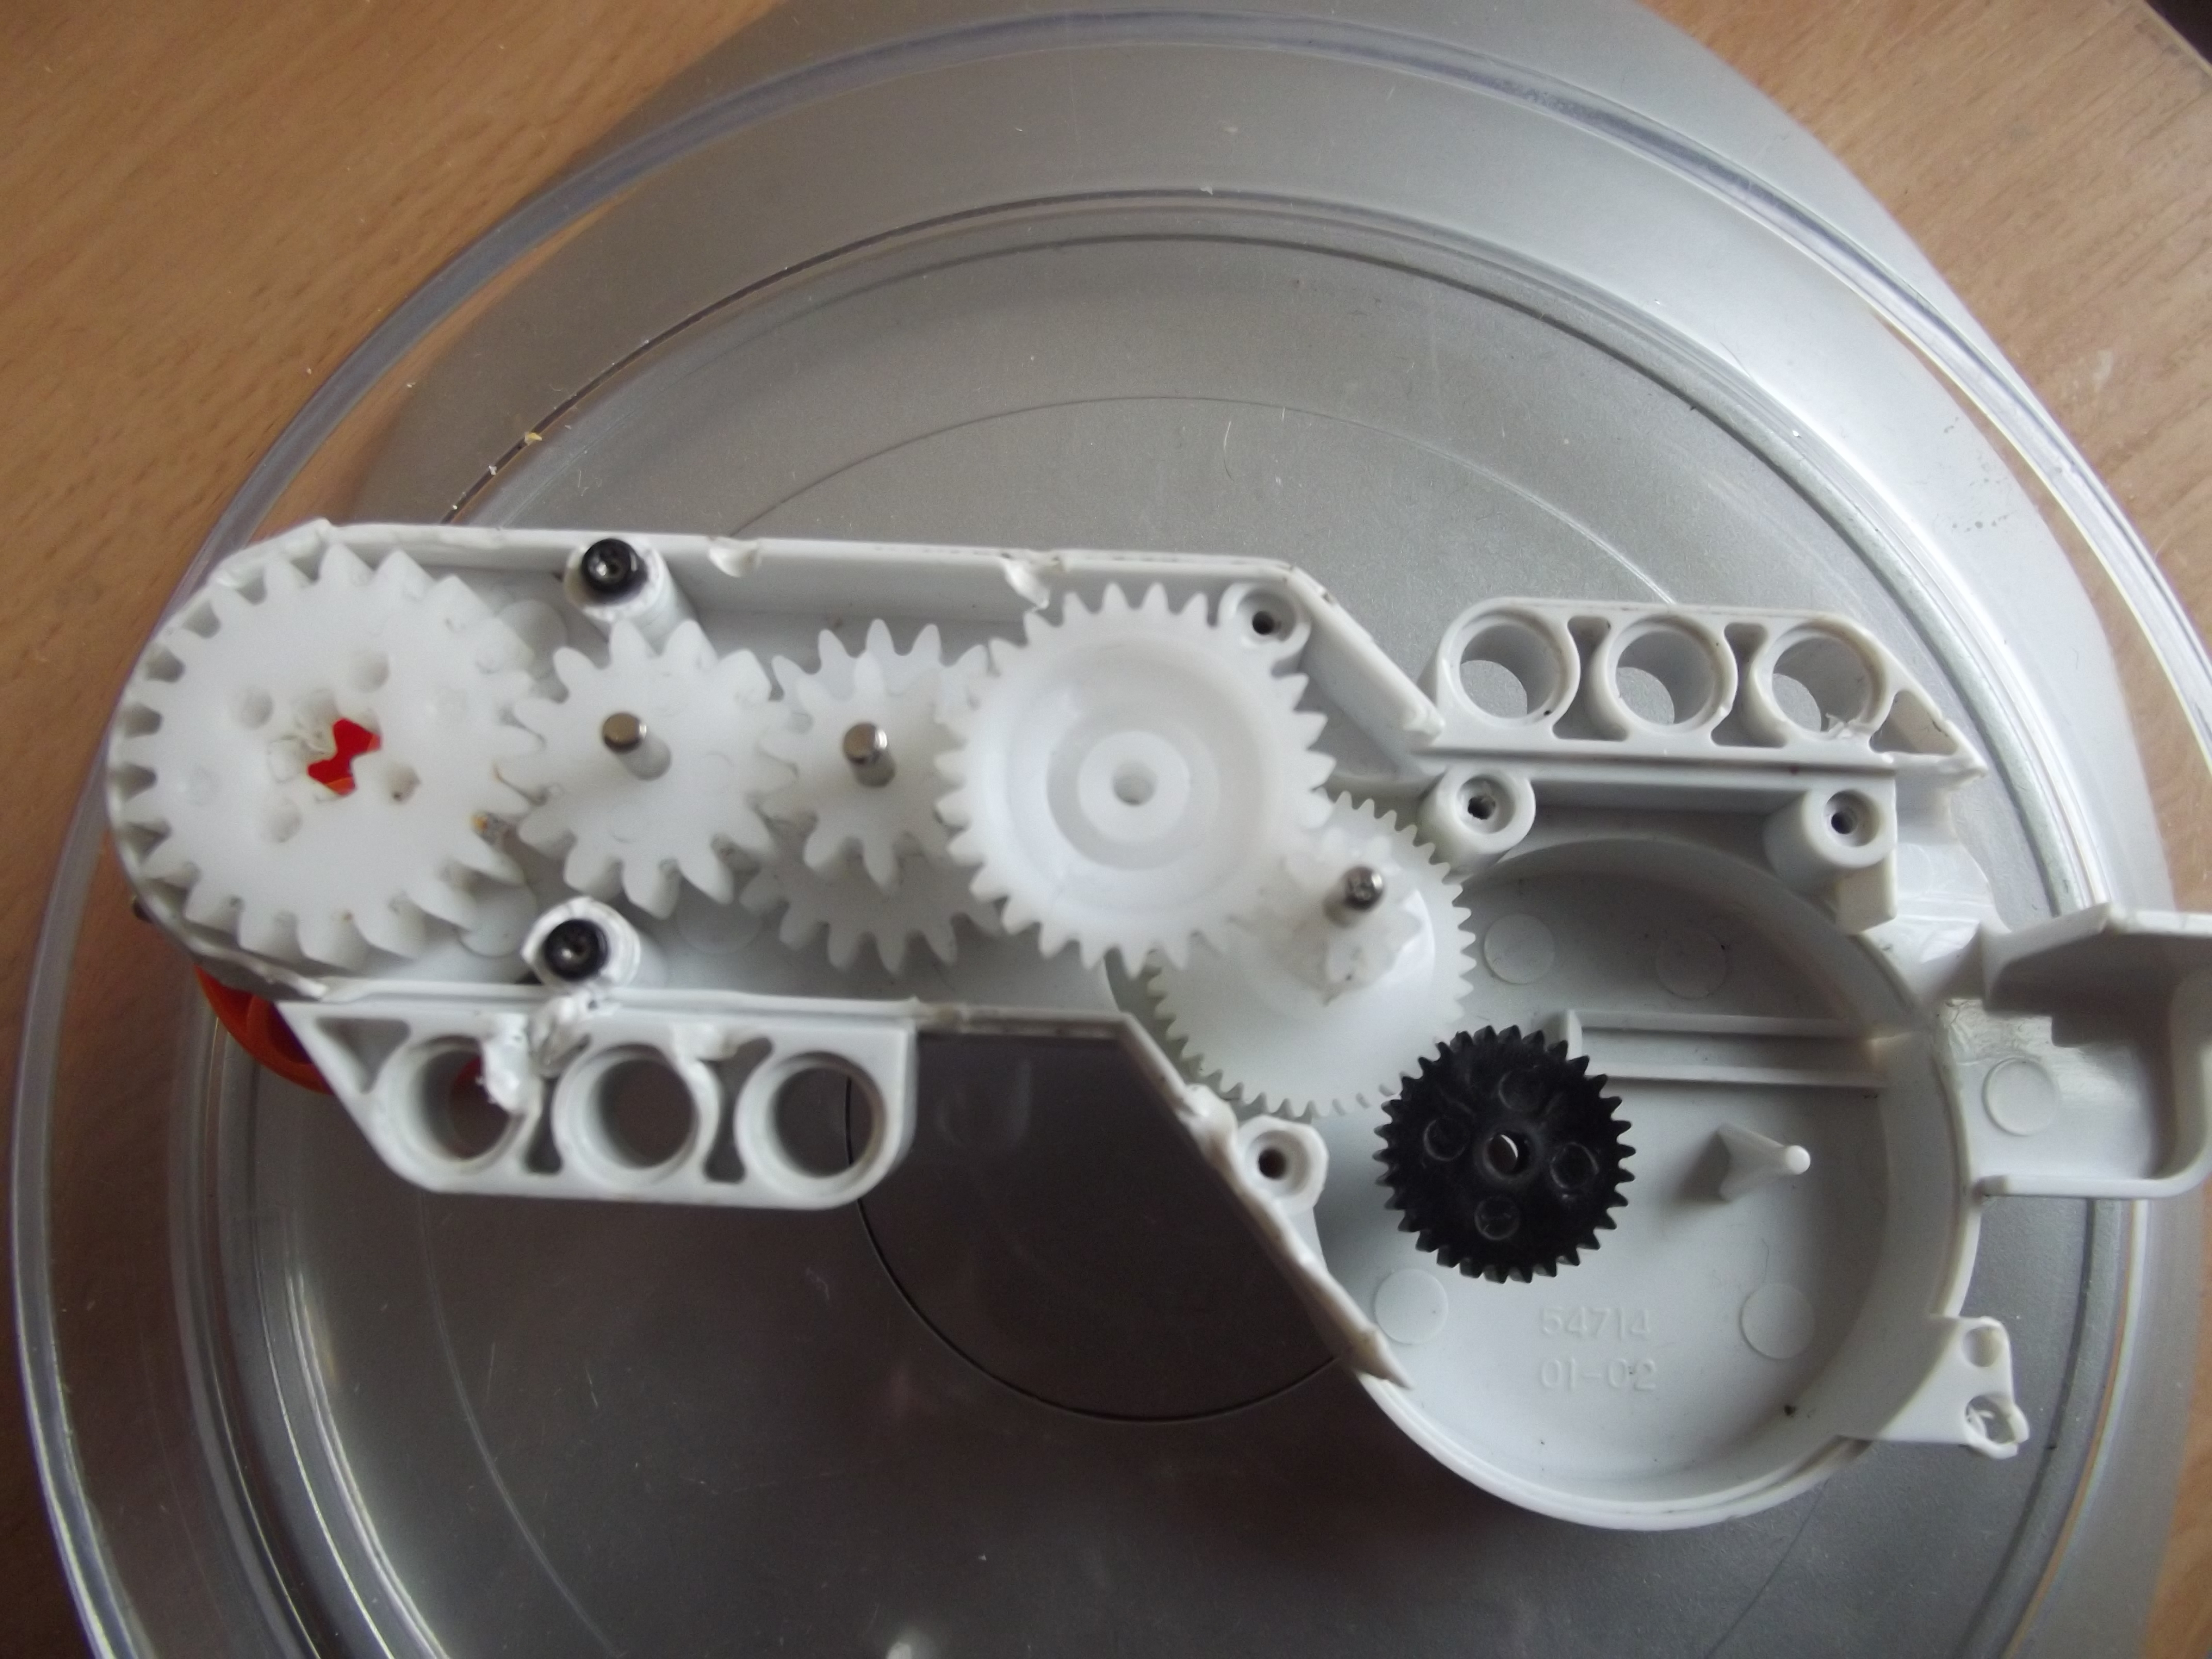
\includegraphics[scale=0.08]{transmition.jpg}
	}
	\caption{Редуктор двигателя NXT.}
	\label{fig:transmition}
\end{figure}

\section{Порядок выполнения работы}

\begin{enumerate}
\item Снятие показаний с двигателя NXT.
	\begin{enumerate}
	\item Соберите конструкцию, такую~же как и в~первой работе.
	\item Реализуйте программу в~среде разработки, которая выполняет следующие действия: организует движения двигателя NXT; выводит на экран значение напряжения выдаваемого аккумулятором.
	\item Скомпилируйте и загрузите программу в~программируемый блок NXT.
	\item Запустите программу.
	\end{enumerate}
\item Определение конструктивных постоянных двигателя NXT.
	\begin{enumerate}
	\item При помощи мультиметра зафиксируйте значения тока, сопротивления и напряжения в~цепи двигателя (не забудьте, что напряжение измеряется на~нагрузке, а ток в~разрыве цепи). Пусковой ток необходимо измерять при застопоренном роторе, для этого зажмите выходной вал рукой.
	\item Также необходимо рассчитать момент инерции ротора двигателя. Для этого измерьте значения массы и диаметра ротора. Используя формулу момента инерции для вращающегося цилиндра, получите чисенное значение.
	\begin{figure}[h]
		\noindent\centering{
			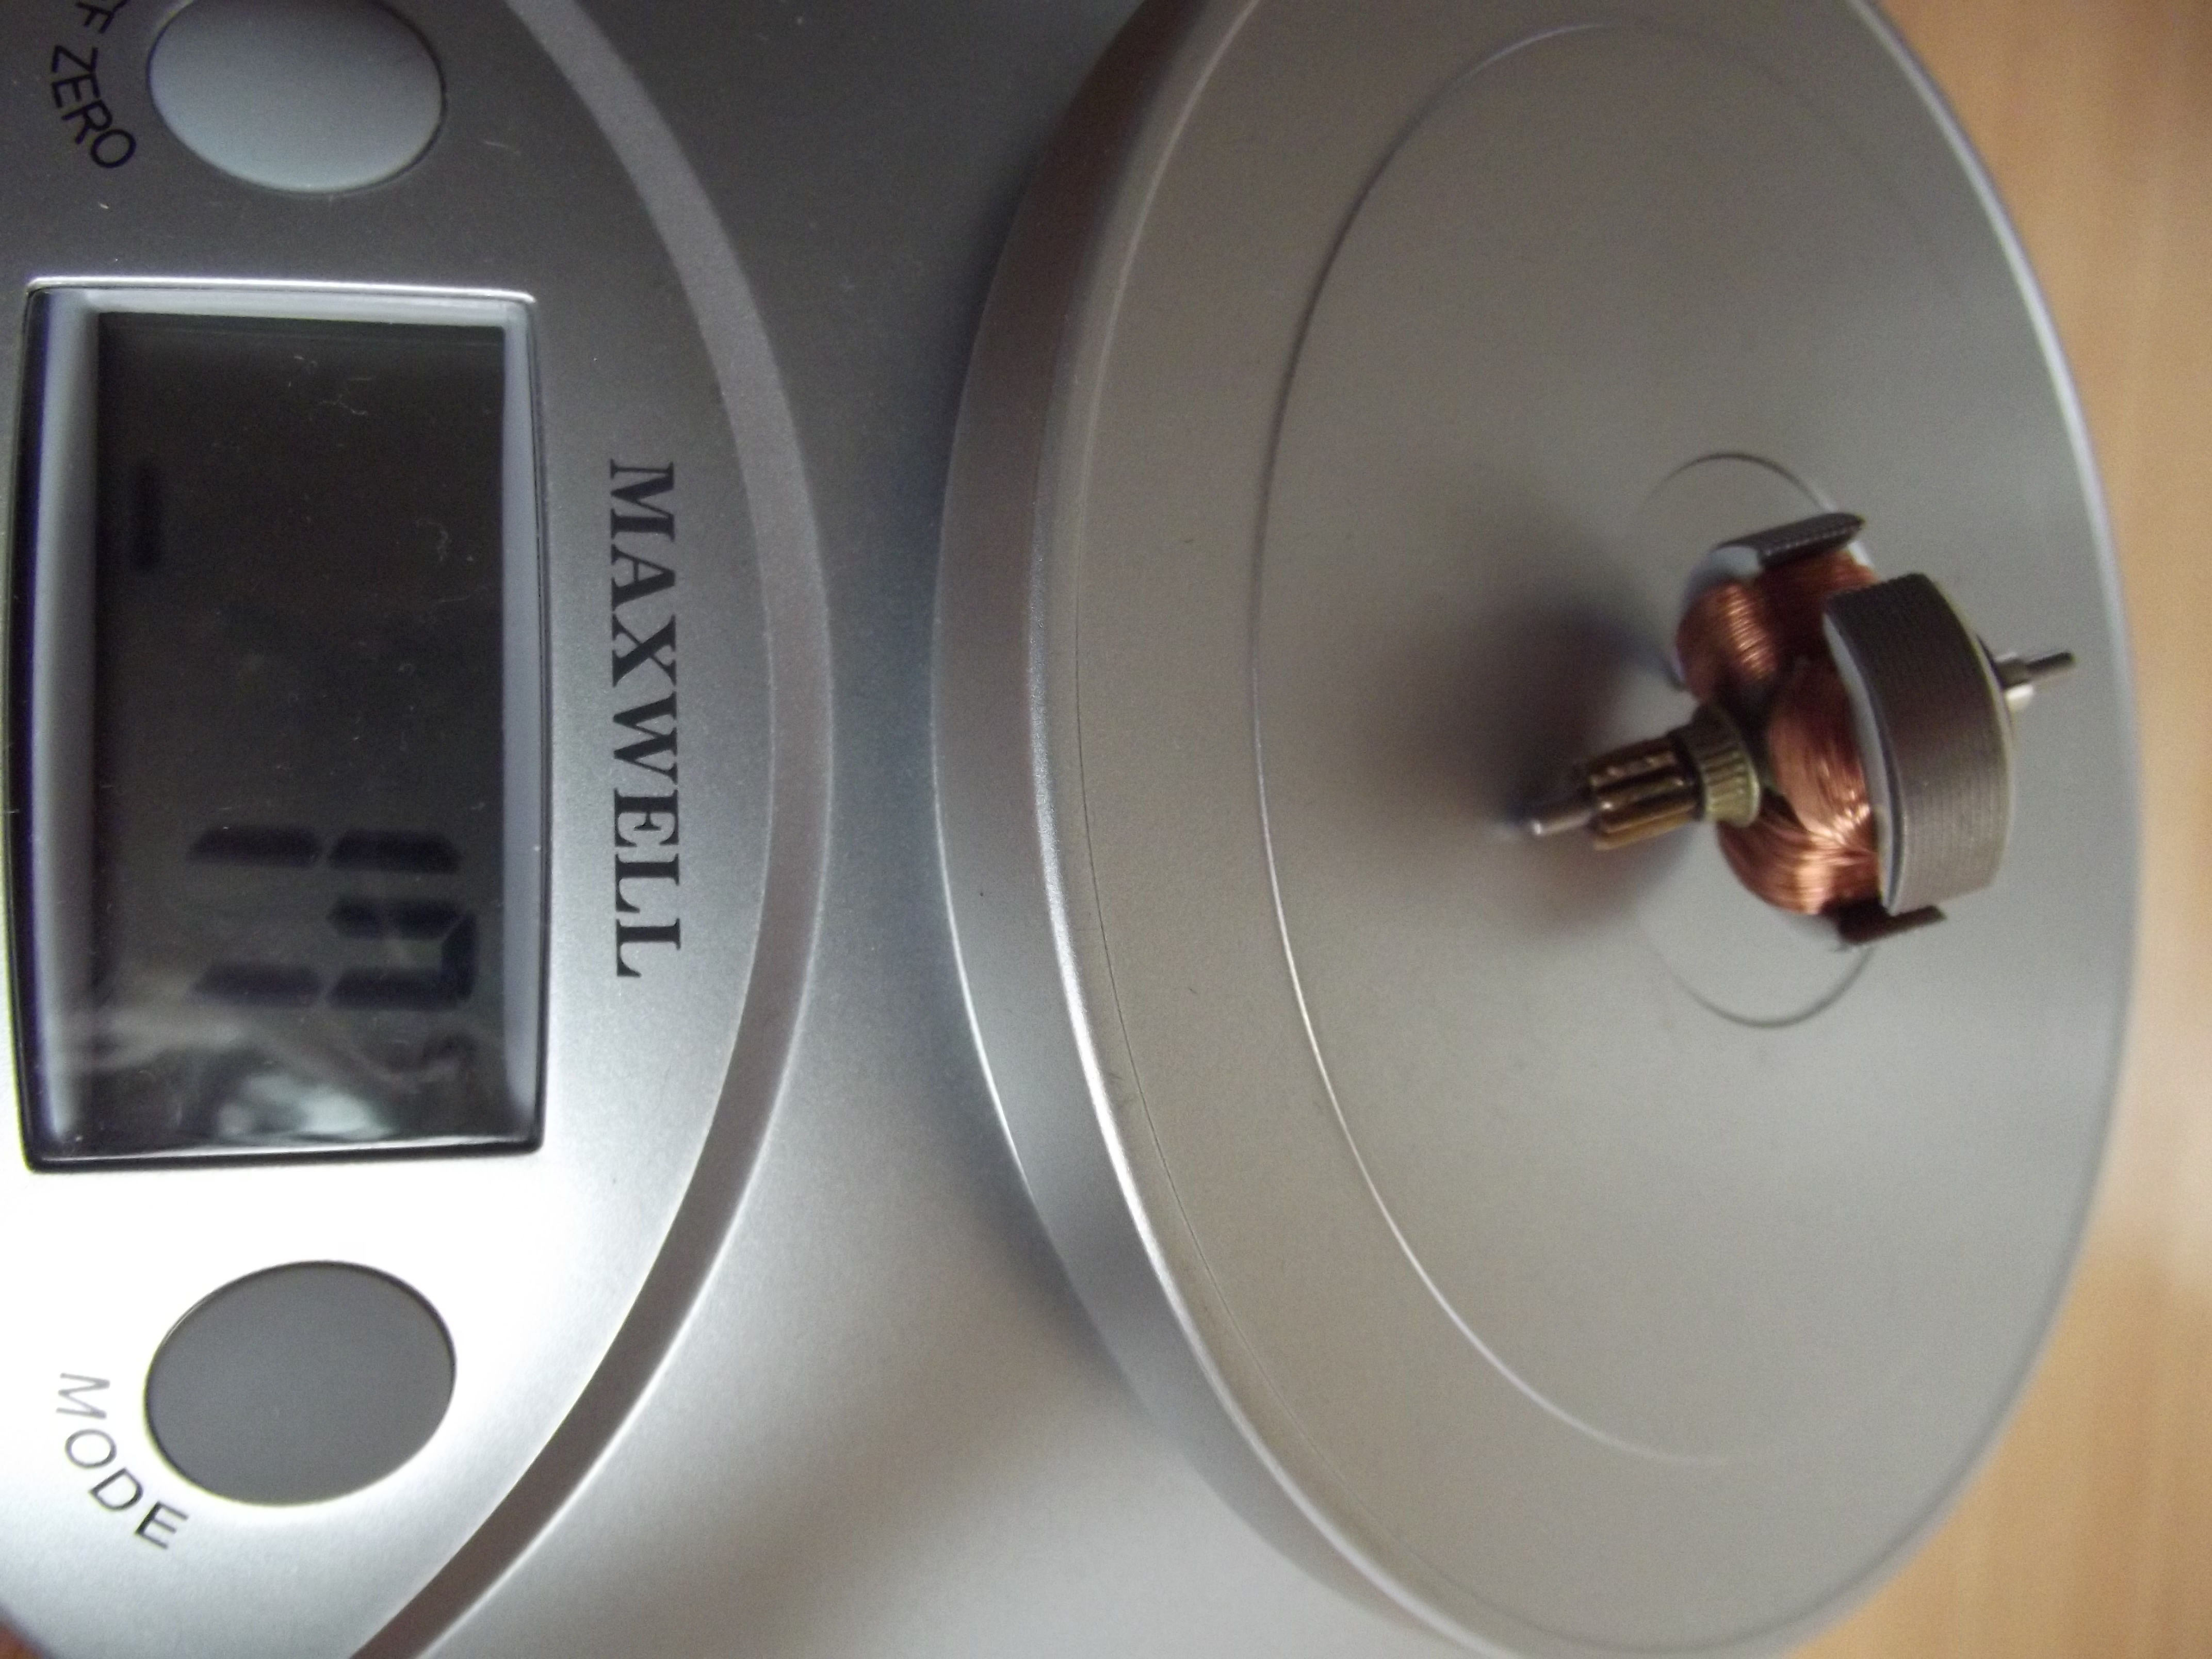
\includegraphics[scale=0.08,angle=90]{rotor.jpg}
		}
		\caption{Ротор двигателя, вес 17 грамм.}
		\label{fig:transmition}
	\end{figure}
	\item Подставив полученные данные (измеренное среднее значение индуктивности 0,0047 Генри), рассчитайте конструктивные постоянные двигателя. Для~этого воспользуйтесь значениями, полученными в~первой работе.
	\item Рассчитанные значения конструктивных постоянных описывают сам двигатель. Для получения характеристик на выходном вале редуктора, конструктивные постоянные нужно домножить на 48, так как момент будет в 48 раз больше, а скорость во столько же раз меньше.
\end{enumerate}
\item Математическое моделирование двигателя.
	\begin{enumerate}
	\item Необходимо сравнить графики переходных процессов при подаче на двигатель ШИМ-сигнала и постоянного напряжения.
	\begin{figure}[h]
		\noindent\centering{
			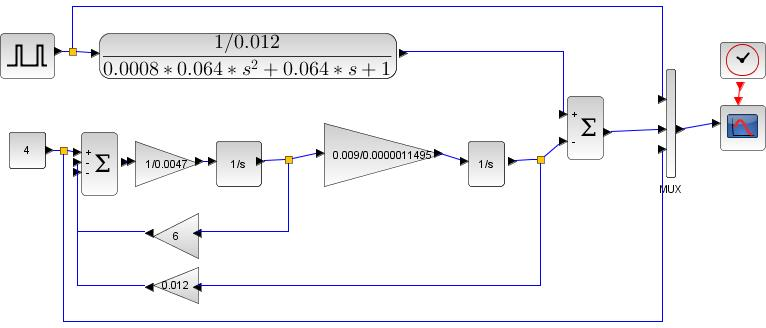
\includegraphics[scale=0.5]{5.jpg}
		}
		\caption{Пример моделирования двигателя в системе Xcos.}
		\label{fig:transmition}
	\end{figure}
	
	\begin{figure}[h]
		\noindent\centering\H{
			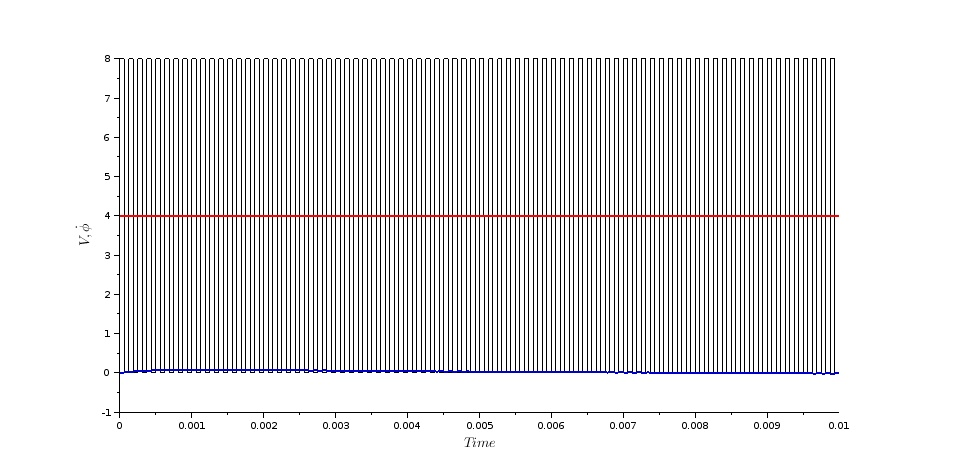
\includegraphics[scale=0.55]{2models.jpeg}
		}
		\caption{Графики задающих воздействий и ошибки в системе Xcos.}
		\label{fig:transmition}
	\end{figure}
	
	\end{enumerate}
\end{enumerate}

\newpage
\section{Содержание отчета}
\begin{enumerate}
\item Исходный код написанной программы.
\item Полученные данные параметров двигателя.
\item Расчеты конструктивных постоянных двигателя.
\item Схема и графики, полученные при~математическом моделировании.
\item Выводы.
\end{enumerate}
\end{document}